\documentclass[11pt,letterpaper]{article}

% =============================================================================
% PACKAGES
% =============================================================================
\usepackage[margin=1in]{geometry}
\usepackage{enumitem}
\usepackage{setspace}
\usepackage{graphicx}
\usepackage{xcolor}
\usepackage{tikz}
\usetikzlibrary{shapes.geometric, arrows.meta, positioning, fit, backgrounds, calc, decorations.pathreplacing, trees, matrix, shapes.multipart, shapes.symbols, petri}
\usepackage{tcolorbox}
\usepackage{booktabs}
\usepackage{longtable}
\usepackage{array}
\usepackage{tabularx}
\usepackage{multirow}
\usepackage{fancyhdr}
\usepackage{titlesec}
\usepackage[colorlinks=true,linkcolor=blue!60!black,urlcolor=blue!60!black,citecolor=blue!60!black]{hyperref}
\usepackage{bookmark}
\usepackage{parskip}
\usepackage{float}
\usepackage{caption}
\usepackage{subcaption}
\usepackage{listings}
\usepackage{microtype}
\usepackage{textcomp}
\usepackage{amssymb}
\usepackage{amsmath}
\usepackage{pifont}

% =============================================================================
% CONFIGURATION
% =============================================================================
\setstretch{1.15}

% Define colors
\definecolor{primary}{RGB}{80, 50, 120}
\definecolor{secondary}{RGB}{100, 80, 140}
\definecolor{accent}{RGB}{200, 80, 60}
\definecolor{success}{RGB}{50, 140, 80}
\definecolor{warning}{RGB}{220, 160, 40}
\definecolor{critical}{RGB}{200, 60, 60}
\definecolor{lightgray}{RGB}{245, 245, 245}
\definecolor{darkgray}{RGB}{80, 80, 80}
\definecolor{processcolor}{RGB}{230, 220, 255}
\definecolor{threadcolor}{RGB}{220, 240, 255}
\definecolor{synccolor}{RGB}{255, 240, 220}
\definecolor{resourcecolor}{RGB}{230, 255, 230}
\definecolor{messagecolor}{RGB}{255, 230, 230}
\definecolor{poolcolor}{RGB}{240, 240, 255}
\definecolor{queuecolor}{RGB}{255, 250, 220}

% Section formatting
\titleformat{\section}{\Large\bfseries\color{primary}}{\thesection}{1em}{}[\titlerule]
\titleformat{\subsection}{\large\bfseries\color{secondary}}{\thesubsection}{1em}{}
\titleformat{\subsubsection}{\normalsize\bfseries\color{darkgray}}{\thesubsubsection}{1em}{}

% Header/Footer
\pagestyle{fancy}
\fancyhf{}
\fancyhead[L]{\small\textcolor{darkgray}{Process Viewpoint Specification}}
\fancyhead[R]{\small\textcolor{darkgray}{Architecture Documentation}}
\fancyfoot[C]{\thepage}
\renewcommand{\headrulewidth}{0.4pt}

% Custom environments
\newtcolorbox{definitionbox}[1][]{
    colback=lightgray,
    colframe=primary,
    fonttitle=\bfseries,
    title=#1,
    boxrule=0.5pt,
    arc=2pt,
    left=8pt,
    right=8pt,
    top=6pt,
    bottom=6pt
}

\newtcolorbox{examplebox}[1][]{
    colback=white,
    colframe=secondary,
    fonttitle=\bfseries,
    title=#1,
    boxrule=0.5pt,
    arc=2pt,
    left=8pt,
    right=8pt,
    top=6pt,
    bottom=6pt
}

\newtcolorbox{warningbox}[1][]{
    colback=orange!5,
    colframe=accent,
    fonttitle=\bfseries,
    title=#1,
    boxrule=0.5pt,
    arc=2pt,
    left=8pt,
    right=8pt,
    top=6pt,
    bottom=6pt
}

\newtcolorbox{guidancebox}[1][]{
    colback=green!5,
    colframe=success,
    fonttitle=\bfseries,
    title=#1,
    boxrule=0.5pt,
    arc=2pt,
    left=8pt,
    right=8pt,
    top=6pt,
    bottom=6pt
}

\newtcolorbox{patternbox}[1][]{
    colback=blue!3,
    colframe=primary!70,
    fonttitle=\bfseries,
    title=#1,
    boxrule=0.5pt,
    arc=2pt,
    left=8pt,
    right=8pt,
    top=6pt,
    bottom=6pt
}

\newtcolorbox{concurrencybox}[1][]{
    colback=purple!5,
    colframe=primary,
    fonttitle=\bfseries,
    title=#1,
    boxrule=0.5pt,
    arc=2pt,
    left=8pt,
    right=8pt,
    top=6pt,
    bottom=6pt
}

\newtcolorbox{hazardbox}[1][]{
    colback=red!5,
    colframe=critical,
    fonttitle=\bfseries,
    title=#1,
    boxrule=0.5pt,
    arc=2pt,
    left=8pt,
    right=8pt,
    top=6pt,
    bottom=6pt
}

% Listings configuration
\lstset{
    basicstyle=\ttfamily\small,
    backgroundcolor=\color{lightgray},
    frame=single,
    framerule=0.5pt,
    rulecolor=\color{darkgray},
    breaklines=true,
    captionpos=b,
    tabsize=2,
    showstringspaces=false,
    numbers=left,
    numberstyle=\tiny\color{darkgray},
    numbersep=5pt,
    xleftmargin=15pt,
    keywordstyle=\color{primary}\bfseries,
    commentstyle=\color{darkgray}\itshape,
    stringstyle=\color{success}
}

\lstdefinelanguage{pseudocode}{
    keywords={process, thread, spawn, fork, join, wait, signal, lock, unlock, acquire, release, send, receive, select, parallel, sequential, atomic, synchronized, async, await, yield, notify, broadcast, barrier, mutex, semaphore, monitor, channel, if, else, while, for, return, try, catch, finally},
    sensitive=true,
    comment=[l]{//},
    morecomment=[s]{/*}{*/},
    morestring=[b]",
    morestring=[b]'
}

% Table column types
\newcolumntype{L}[1]{>{\raggedright\arraybackslash}p{#1}}
\newcolumntype{C}[1]{>{\centering\arraybackslash}p{#1}}
\newcolumntype{R}[1]{>{\raggedleft\arraybackslash}p{#1}}

% Custom commands
\newcommand{\cmark}{\ding{51}}
\newcommand{\xmark}{\ding{55}}

% =============================================================================
% DOCUMENT BEGIN
% =============================================================================
\begin{document}

% -----------------------------------------------------------------------------
% TITLE PAGE
% -----------------------------------------------------------------------------
\hypersetup{pageanchor=false}
\begin{titlepage}
    \centering
    \vspace*{1.5cm}
    
    {\Huge\bfseries\color{primary} Process Viewpoint\par}
    \vspace{0.5cm}
    {\Large\color{secondary} Architecture Viewpoint Specification\par}
    \vspace{0.3cm}
    {\large\color{darkgray} Concurrency, Parallelism \& Runtime Behavior\par}
    
    \vspace{1.3cm}
    
    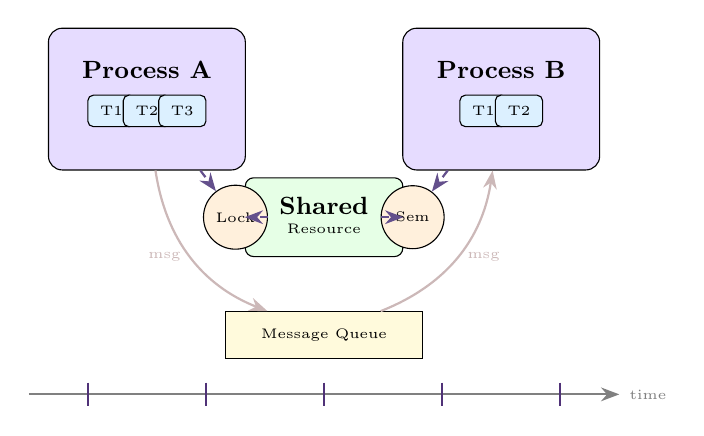
\begin{tikzpicture}[scale=0.75]
        % Process 1
        \node[draw, rounded corners=5pt, fill=processcolor, minimum width=2.5cm, minimum height=1.8cm] (p1) at (-3, 2) {};
        \node[font=\small\bfseries] at (-3, 2.5) {Process A};
        \node[draw, fill=threadcolor, rounded corners=2pt, minimum width=0.6cm, minimum height=0.4cm, font=\tiny] at (-3.6, 1.8) {T1};
        \node[draw, fill=threadcolor, rounded corners=2pt, minimum width=0.6cm, minimum height=0.4cm, font=\tiny] at (-3, 1.8) {T2};
        \node[draw, fill=threadcolor, rounded corners=2pt, minimum width=0.6cm, minimum height=0.4cm, font=\tiny] at (-2.4, 1.8) {T3};
        
        % Process 2
        \node[draw, rounded corners=5pt, fill=processcolor, minimum width=2.5cm, minimum height=1.8cm] (p2) at (3, 2) {};
        \node[font=\small\bfseries] at (3, 2.5) {Process B};
        \node[draw, fill=threadcolor, rounded corners=2pt, minimum width=0.6cm, minimum height=0.4cm, font=\tiny] at (2.7, 1.8) {T1};
        \node[draw, fill=threadcolor, rounded corners=2pt, minimum width=0.6cm, minimum height=0.4cm, font=\tiny] at (3.3, 1.8) {T2};
        
        % Shared Resource
        \node[draw, fill=resourcecolor, rounded corners=3pt, minimum width=2cm, minimum height=1cm] (resource) at (0, 0) {};
        \node[font=\small\bfseries] at (0, 0.2) {Shared};
        \node[font=\tiny] at (0, -0.2) {Resource};
        
        % Message Queue
        \node[draw, fill=queuecolor, minimum width=2.5cm, minimum height=0.6cm] (queue) at (0, -2) {};
        \node[font=\tiny] at (0, -2) {Message Queue};
        
        % Synchronization
        \node[draw, fill=synccolor, circle, minimum size=0.8cm, font=\tiny] (lock) at (-1.5, 0) {Lock};
        \node[draw, fill=synccolor, circle, minimum size=0.8cm, font=\tiny] (sem) at (1.5, 0) {Sem};
        
        % Connections
        \draw[-{Stealth}, thick, dashed, secondary] (p1) -- (lock);
        \draw[-{Stealth}, thick, dashed, secondary] (lock) -- (resource);
        \draw[-{Stealth}, thick, dashed, secondary] (p2) -- (sem);
        \draw[-{Stealth}, thick, dashed, secondary] (sem) -- (resource);
        
        % Message passing
        \draw[-{Stealth}, thick, messagecolor!80!black] (p1) to[bend right=30] node[midway, left, font=\tiny] {msg} (queue);
        \draw[-{Stealth}, thick, messagecolor!80!black] (queue) to[bend right=30] node[midway, right, font=\tiny] {msg} (p2);
        
        % Timeline indicator
        \draw[-{Stealth}, thick, gray] (-5, -3) -- (5, -3) node[right, font=\tiny] {time};
        \draw[thick, primary] (-4, -2.8) -- (-4, -3.2);
        \draw[thick, primary] (-2, -2.8) -- (-2, -3.2);
        \draw[thick, primary] (0, -2.8) -- (0, -3.2);
        \draw[thick, primary] (2, -2.8) -- (2, -3.2);
        \draw[thick, primary] (4, -2.8) -- (4, -3.2);
    \end{tikzpicture}
    
    \vspace{1.5cm}
    
    \begin{tabular}{ll}
        \textbf{Version:} & 2.0 \\
        \textbf{Status:} & Release \\
        \textbf{Classification:} & ISO/IEC/IEEE 42010 Compliant \\
        \textbf{Last Updated:} & \today \\
    \end{tabular}
    
    \vfill
    
    {\small Based on the Views and Beyond approach to software architecture documentation}
    
\end{titlepage}
\clearpage
\hypersetup{pageanchor=true}

% -----------------------------------------------------------------------------
% TABLE OF CONTENTS
% -----------------------------------------------------------------------------
\tableofcontents
\newpage

% =============================================================================
% SECTION: VIEWPOINT NAME
% =============================================================================
\section{Viewpoint Name}

\begin{definitionbox}[Viewpoint Identification]
\begin{tabular}{@{}L{3.5cm}L{10cm}@{}}
\textbf{Name:} & Process Viewpoint \\[0.5em]
\textbf{Synonyms:} & Concurrency Viewpoint, Runtime Viewpoint, Thread View, Execution View, Dynamic View, Behavioral View, Parallel Processing View \\[0.5em]
\textbf{Identifier:} & VP-PROC-001 \\[0.5em]
\textbf{Version:} & 2.0 \\
\end{tabular}
\end{definitionbox}

\subsection{Viewpoint Classification}

The Process Viewpoint addresses the runtime structure of a system in terms of processes, threads, and their interactions. Within the Views and Beyond approach, this corresponds to Component-and-Connector (C\&C) views that emphasize runtime elements, particularly the Communicating Processes style. This viewpoint is essential for understanding how a system achieves parallelism, manages concurrency, and coordinates distributed execution.

\begin{table}[H]
\centering
\caption{Viewpoint Classification Taxonomy}
\begin{tabular}{@{}L{4cm}L{10cm}@{}}
\toprule
\textbf{Attribute} & \textbf{Value} \\
\midrule
Style Family & Component-and-Connector (C\&C) \\
Primary Focus & Runtime Processes, Threads, and Coordination \\
Abstraction Level & Runtime / Execution \\
Temporal Perspective & Dynamic Behavior Over Time \\
Related Styles & Communicating Processes, Shared-Data, Client-Server \\
IEEE 42010 Category & Concurrency Viewpoint \\
4+1 View Model & Process View \\
\bottomrule
\end{tabular}
\end{table}

\subsection{Viewpoint Scope}

The Process Viewpoint encompasses multiple aspects of runtime behavior:

\begin{itemize}
    \item \textbf{Process Structure:} Operating system processes, their boundaries, and lifecycle management.
    
    \item \textbf{Thread Architecture:} Thread organization within processes, thread pools, and worker patterns.
    
    \item \textbf{Concurrency Control:} Mechanisms for coordinating concurrent access to shared resources including locks, semaphores, monitors, and transactions.
    
    \item \textbf{Inter-Process Communication:} How processes exchange data through shared memory, message passing, pipes, sockets, and other IPC mechanisms.
    
    \item \textbf{Synchronization:} Coordination points where processes or threads must synchronize their execution.
    
    \item \textbf{Parallelism:} How work is distributed across multiple processing units for performance.
    
    \item \textbf{Scheduling:} How processing resources are allocated to competing tasks.
    
    \item \textbf{State Management:} How state is managed across concurrent execution paths.
\end{itemize}

% =============================================================================
% SECTION: OVERVIEW
% =============================================================================
\section{Overview}

The Process Viewpoint provides a comprehensive framework for documenting the runtime execution structure of a software system. It addresses how the system leverages concurrent and parallel execution, manages shared resources safely, and coordinates activities across multiple execution contexts.

\subsection{Purpose and Scope}

The primary purpose of this viewpoint is to establish a clear understanding of the system's runtime topology in terms of processes and threads, the mechanisms used for coordination and communication, and the strategies employed to achieve required performance and reliability characteristics in a concurrent environment.

\begin{definitionbox}[Viewpoint Definition]
The Process Viewpoint defines the runtime structure of a system in terms of processes, threads, and other units of execution. It documents how these execution units are organized, how they communicate and synchronize, and how they share resources. This viewpoint addresses concerns of concurrency, parallelism, performance, scalability, and fault tolerance at runtime.
\end{definitionbox}

\subsection{Key Characteristics}

The Process Viewpoint exhibits several distinctive characteristics:

\textbf{Runtime Focus:} Unlike module views that show static structure, this viewpoint shows runtime entities that exist during execution and may be created/destroyed dynamically.

\textbf{Temporal Dimension:} Processes and threads execute over time, making temporal ordering, synchronization points, and timing constraints essential aspects of documentation.

\textbf{Non-Determinism:} Concurrent systems can exhibit non-deterministic behavior due to scheduling, making analysis of possible interleavings important.

\textbf{Resource Contention:} Multiple execution units competing for shared resources requires explicit documentation of contention management.

\textbf{Scalability Implications:} Process and thread architecture directly impacts system scalability and performance under load.

\subsection{Relationship to Other Viewpoints}

The Process Viewpoint connects to other architectural viewpoints in significant ways:

\begin{table}[H]
\centering
\caption{Relationships to Other Viewpoints}
\begin{tabular}{@{}L{3.5cm}L{10.5cm}@{}}
\toprule
\textbf{Viewpoint} & \textbf{Relationship} \\
\midrule
Development & Code modules are packaged into processes. Thread implementations reside in modules. \\
\addlinespace
Deployment & Processes execute on nodes. Thread pools size based on hardware. Process distribution across nodes. \\
\addlinespace
Component-and-Connector & Processes are runtime manifestations of components. Connectors implement IPC. \\
\addlinespace
Information/Data & Data stores are accessed concurrently. Transactions coordinate data access. \\
\addlinespace
Operational & Process monitoring, scaling policies, resource management. \\
\addlinespace
Security & Process isolation, privilege separation, secure IPC. \\
\bottomrule
\end{tabular}
\end{table}

\subsection{Concurrency Architecture Overview}

\begin{figure}[H]
\centering
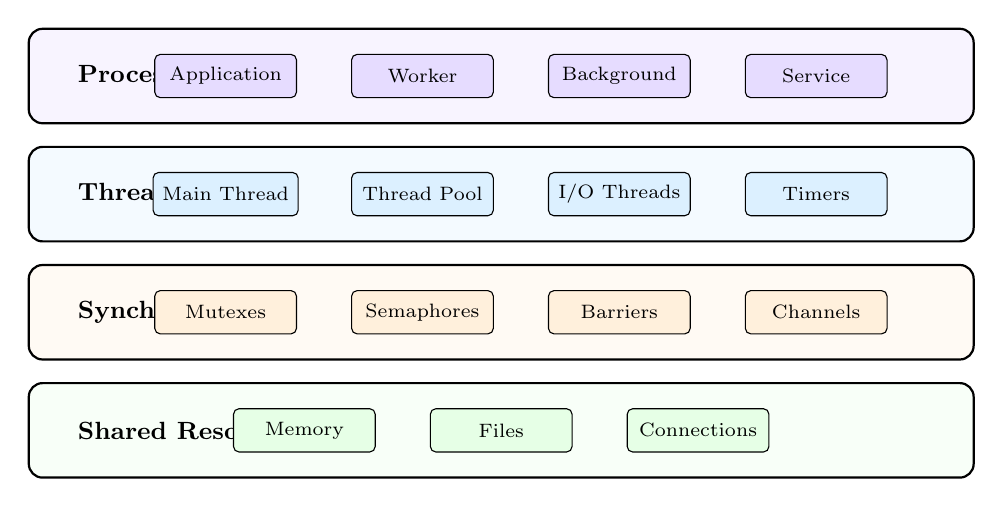
\begin{tikzpicture}[
    node distance=1cm and 1.5cm,
    layer/.style={draw, thick, rounded corners=5pt, minimum width=12cm, minimum height=1.2cm, font=\small},
    element/.style={draw, fill=processcolor, rounded corners=2pt, minimum width=1.8cm, minimum height=0.55cm, font=\scriptsize},
    arrow/.style={-{Stealth}, thick, gray}
]
    % Layers
    \node[layer, fill=processcolor!30] (process) at (0, 3.5) {};
    \node[font=\small\bfseries, anchor=west] at (-5.5, 3.5) {Process Layer};
    
    \node[layer, fill=threadcolor!30] (thread) at (0, 2) {};
    \node[font=\small\bfseries, anchor=west] at (-5.5, 2) {Thread Layer};
    
    \node[layer, fill=synccolor!30] (sync) at (0, 0.5) {};
    \node[font=\small\bfseries, anchor=west] at (-5.5, 0.5) {Synchronization};
    
    \node[layer, fill=resourcecolor!30] (resource) at (0, -1) {};
    \node[font=\small\bfseries, anchor=west] at (-5.5, -1) {Shared Resources};
    
    % Process elements
    \node[element] at (-3.5, 3.5) {Application};
    \node[element] at (-1, 3.5) {Worker};
    \node[element] at (1.5, 3.5) {Background};
    \node[element] at (4, 3.5) {Service};
    
    % Thread elements
    \node[element, fill=threadcolor] at (-3.5, 2) {Main Thread};
    \node[element, fill=threadcolor] at (-1, 2) {Thread Pool};
    \node[element, fill=threadcolor] at (1.5, 2) {I/O Threads};
    \node[element, fill=threadcolor] at (4, 2) {Timers};
    
    % Sync elements
    \node[element, fill=synccolor] at (-3.5, 0.5) {Mutexes};
    \node[element, fill=synccolor] at (-1, 0.5) {Semaphores};
    \node[element, fill=synccolor] at (1.5, 0.5) {Barriers};
    \node[element, fill=synccolor] at (4, 0.5) {Channels};
    
    % Resource elements
    \node[element, fill=resourcecolor] at (-2.5, -1) {Memory};
    \node[element, fill=resourcecolor] at (0, -1) {Files};
    \node[element, fill=resourcecolor] at (2.5, -1) {Connections};
    
\end{tikzpicture}
\caption{Concurrency Architecture Layers}
\end{figure}

% =============================================================================
% SECTION: CONCERNS
% =============================================================================
\section{Concerns}

This section enumerates the architectural concerns that the Process Viewpoint is designed to address.

\subsection{Primary Concerns}

\begin{enumerate}[label=\textbf{C\arabic*:}, leftmargin=2.5em]
    \item \textbf{Process Organization}
    \begin{itemize}[nosep]
        \item What are the major processes in the system?
        \item How are processes organized and related?
        \item What is the lifecycle of each process?
        \item How are processes created, managed, and terminated?
        \item What isolation boundaries exist between processes?
    \end{itemize}
    
    \item \textbf{Thread Architecture}
    \begin{itemize}[nosep]
        \item How are threads organized within processes?
        \item What threading models are used (one-per-request, thread pool, event loop)?
        \item How are thread pools sized and managed?
        \item What thread-local storage is used?
        \item How is thread lifecycle managed?
    \end{itemize}
    
    \item \textbf{Concurrency Control}
    \begin{itemize}[nosep]
        \item What shared resources require protection?
        \item What synchronization mechanisms are used?
        \item How is deadlock prevented or detected?
        \item What locking granularity is employed?
        \item How is lock contention minimized?
    \end{itemize}
    
    \item \textbf{Inter-Process Communication}
    \begin{itemize}[nosep]
        \item How do processes communicate?
        \item What IPC mechanisms are used (shared memory, messages, pipes)?
        \item What message formats and protocols are employed?
        \item How is communication reliability ensured?
        \item What are the communication patterns (sync/async, unicast/multicast)?
    \end{itemize}
    
    \item \textbf{Parallelism and Performance}
    \begin{itemize}[nosep]
        \item How is work partitioned for parallel execution?
        \item What parallel algorithms or patterns are used?
        \item How does the system scale with additional processors?
        \item What are the performance bottlenecks?
        \item How is load balanced across execution units?
    \end{itemize}
    
    \item \textbf{Scheduling and Priority}
    \begin{itemize}[nosep]
        \item How are tasks scheduled for execution?
        \item What priority schemes are used?
        \item How is fairness ensured?
        \item What real-time constraints exist?
        \item How is scheduling latency managed?
    \end{itemize}
    
    \item \textbf{State Management}
    \begin{itemize}[nosep]
        \item What state is shared between execution units?
        \item How is state consistency maintained?
        \item What isolation levels are provided?
        \item How is distributed state coordinated?
        \item What happens to state during failures?
    \end{itemize}
    
    \item \textbf{Fault Tolerance}
    \begin{itemize}[nosep]
        \item How does the system handle process failures?
        \item What supervision and restart strategies exist?
        \item How are partial failures handled?
        \item What failure isolation boundaries exist?
        \item How is system consistency maintained after failures?
    \end{itemize}
    
    \item \textbf{Resource Management}
    \begin{itemize}[nosep]
        \item How are system resources (CPU, memory, connections) allocated?
        \item What resource limits and quotas exist?
        \item How is resource exhaustion prevented?
        \item What cleanup mechanisms ensure resource release?
        \item How are resources pooled and reused?
    \end{itemize}
    
    \item \textbf{Determinism and Reproducibility}
    \begin{itemize}[nosep]
        \item How deterministic is system behavior?
        \item What sources of non-determinism exist?
        \item How is testing of concurrent behavior performed?
        \item What debugging support exists for concurrency issues?
        \item How are race conditions detected and prevented?
    \end{itemize}
\end{enumerate}

\subsection{Concern-Quality Attribute Mapping}

\begin{table}[H]
\centering
\caption{Concern to Quality Attribute Mapping}
\small
\begin{tabular}{@{}L{3cm}C{1cm}C{1cm}C{1cm}C{1cm}C{1cm}C{1cm}C{1cm}C{1cm}@{}}
\toprule
\textbf{Concern} & \rotatebox{60}{\textbf{Performance}} & \rotatebox{60}{\textbf{Scalability}} & \rotatebox{60}{\textbf{Reliability}} & \rotatebox{60}{\textbf{Availability}} & \rotatebox{60}{\textbf{Security}} & \rotatebox{60}{\textbf{Maintaintic.}} & \rotatebox{60}{\textbf{Testability}} & \rotatebox{60}{\textbf{Safety}} \\
\midrule
Process Org. & $\circ$ & $\bullet$ & $\bullet$ & $\bullet$ & $\bullet$ & $\circ$ & $\circ$ & $\circ$ \\
Thread Arch. & $\bullet$ & $\bullet$ & $\circ$ & $\circ$ & $\circ$ & $\circ$ & $\circ$ & $\circ$ \\
Concurrency & $\bullet$ & $\circ$ & $\bullet$ & $\circ$ & $\circ$ & $\circ$ & $\circ$ & $\bullet$ \\
IPC & $\bullet$ & $\bullet$ & $\circ$ & $\circ$ & $\bullet$ & $\circ$ & $\circ$ & -- \\
Parallelism & $\bullet$ & $\bullet$ & $\circ$ & -- & -- & $\circ$ & $\circ$ & -- \\
Scheduling & $\bullet$ & $\circ$ & $\circ$ & $\circ$ & -- & -- & -- & $\bullet$ \\
State Mgmt & $\circ$ & $\circ$ & $\bullet$ & $\circ$ & $\circ$ & $\circ$ & $\circ$ & $\bullet$ \\
Fault Tol. & -- & $\circ$ & $\bullet$ & $\bullet$ & -- & $\circ$ & $\circ$ & $\bullet$ \\
Resources & $\bullet$ & $\bullet$ & $\bullet$ & $\bullet$ & $\circ$ & $\circ$ & -- & -- \\
Determinism & $\circ$ & -- & $\circ$ & -- & -- & $\circ$ & $\bullet$ & $\bullet$ \\
\bottomrule
\multicolumn{9}{l}{\footnotesize $\bullet$ = Primary impact, $\circ$ = Secondary impact, -- = Minimal impact}
\end{tabular}
\end{table}

% =============================================================================
% SECTION: ANTI-CONCERNS
% =============================================================================
\section{Anti-Concerns}

Understanding what the Process Viewpoint is \emph{not} appropriate for helps stakeholders avoid misapplying this viewpoint.

\subsection{Out of Scope Topics}

\begin{enumerate}[label=\textbf{AC\arabic*:}, leftmargin=2.5em]
    \item \textbf{Static Code Structure}
    \begin{itemize}[nosep]
        \item Module organization and dependencies
        \item Class hierarchies and inheritance
        \item Package structure and namespaces
        \item Build dependencies
        \item Code file organization
    \end{itemize}
    
    \item \textbf{Physical Deployment}
    \begin{itemize}[nosep]
        \item Hardware specifications
        \item Network topology
        \item Container orchestration
        \item Cloud infrastructure
        \item Data center design
    \end{itemize}
    
    \item \textbf{Data Modeling}
    \begin{itemize}[nosep]
        \item Entity-relationship models
        \item Database schema design
        \item Data flow diagrams (except IPC data)
        \item Data retention policies
        \item Data quality rules
    \end{itemize}
    
    \item \textbf{User Interface}
    \begin{itemize}[nosep]
        \item Screen layouts and designs
        \item User interaction flows
        \item Accessibility features
        \item Responsive design
        \item UI component architecture
    \end{itemize}
    
    \item \textbf{Business Logic Details}
    \begin{itemize}[nosep]
        \item Algorithmic implementations
        \item Business rules specifications
        \item Domain model details
        \item Validation logic
        \item Calculation formulas
    \end{itemize}
\end{enumerate}

\begin{warningbox}[Common Misapplications]
Avoid using the Process Viewpoint for:

\begin{itemize}[nosep]
    \item Documenting code module dependencies (use Development Viewpoint)
    \item Specifying server topology (use Deployment Viewpoint)
    \item Defining data schemas (use Information Viewpoint)
    \item Detailing API contracts (use Interface Specifications)
    \item Specifying functional requirements (use Functional Viewpoint)
\end{itemize}
\end{warningbox}

% =============================================================================
% SECTION: TYPICAL STAKEHOLDERS
% =============================================================================
\section{Typical Stakeholders}

The Process Viewpoint serves multiple stakeholder communities with concerns about system runtime behavior.

\subsection{Primary Stakeholders}

\begin{table}[H]
\centering
\caption{Primary Stakeholder Analysis}
\small
\begin{tabular}{@{}L{2.6cm}L{3.6cm}L{7cm}@{}}
\toprule
\textbf{Stakeholder} & \textbf{Role Description} & \textbf{Primary Interests} \\
\midrule
Software Architects & Design system structure & Process topology, IPC mechanisms, concurrency strategy, scalability \\
\addlinespace
Performance Engineers & Optimize system performance & Thread pools, parallelism, contention, bottleneck analysis \\
\addlinespace
Senior Developers & Implement concurrent code & Synchronization primitives, thread safety, deadlock avoidance \\
\addlinespace
Platform Engineers & Manage runtime platform & Process management, resource allocation, scheduling \\
\addlinespace
QA/Test Engineers & Validate concurrent behavior & Race condition testing, stress testing, determinism \\
\addlinespace
System Integrators & Connect system components & IPC protocols, message formats, integration patterns \\
\bottomrule
\end{tabular}
\end{table}

\subsection{Secondary Stakeholders}

\begin{table}[H]
\centering
\caption{Secondary Stakeholder Analysis}
\small
\begin{tabular}{@{}L{2.6cm}L{3.6cm}L{7cm}@{}}
\toprule
\textbf{Stakeholder} & \textbf{Role Description} & \textbf{Primary Interests} \\
\midrule
Operations Teams & Manage production systems & Process monitoring, resource usage, failure recovery \\
\addlinespace
Security Architects & Ensure system security & Process isolation, privilege separation, secure IPC \\
\addlinespace
Capacity Planners & Plan system resources & Thread scaling, process distribution, resource requirements \\
\addlinespace
Real-Time Engineers & Ensure timing constraints & Scheduling, latency, determinism, priority inversion \\
\addlinespace
Embedded Engineers & Develop constrained systems & Resource-limited concurrency, interrupt handling \\
\addlinespace
Technical Managers & Oversee development & Risk assessment, complexity management, skill requirements \\
\bottomrule
\end{tabular}
\end{table}

\subsection{Stakeholder Concern Matrix}

\begin{table}[H]
\centering
\caption{Stakeholder-Concern Responsibility Matrix}
\footnotesize
\begin{tabular}{@{}L{2cm}C{0.8cm}C{0.8cm}C{0.8cm}C{0.8cm}C{0.8cm}C{0.8cm}C{0.8cm}C{0.8cm}C{0.8cm}C{0.8cm}@{}}
\toprule
& \rotatebox{60}{\textbf{Process}} & \rotatebox{60}{\textbf{Thread}} & \rotatebox{60}{\textbf{Concurr.}} & \rotatebox{60}{\textbf{IPC}} & \rotatebox{60}{\textbf{Parallel}} & \rotatebox{60}{\textbf{Schedule}} & \rotatebox{60}{\textbf{State}} & \rotatebox{60}{\textbf{Fault}} & \rotatebox{60}{\textbf{Resource}} & \rotatebox{60}{\textbf{Determ.}} \\
\midrule
Architect & R & R & A & R & A & C & A & A & C & C \\
Perf. Eng. & C & R & C & C & R & R & C & I & R & C \\
Developer & C & A & R & A & C & I & R & C & C & R \\
Platform & A & C & I & C & C & A & I & R & A & I \\
QA/Test & I & C & C & C & I & I & C & C & I & R \\
Security & C & I & C & A & I & I & C & C & C & I \\
\bottomrule
\multicolumn{11}{l}{\footnotesize R = Responsible, A = Accountable, C = Consulted, I = Informed}
\end{tabular}
\end{table}

% =============================================================================
% SECTION: MODEL TYPES
% =============================================================================
\section{Model Types}

The Process Viewpoint employs several complementary model types to capture different aspects of concurrent system structure and behavior.

\subsection{Model Type Catalog}

\begin{enumerate}[label=\textbf{MT\arabic*:}, leftmargin=2.5em]
    \item \textbf{Process Structure Diagram}
    \begin{itemize}[nosep]
        \item \textit{Purpose:} Show processes, their relationships, and communication paths
        \item \textit{Primary Elements:} Processes, threads, communication channels
        \item \textit{Key Relationships:} Communicates-with, spawns, supervises
        \item \textit{Typical Notation:} UML component diagrams, custom process diagrams
    \end{itemize}
    
    \item \textbf{Thread Pool Model}
    \begin{itemize}[nosep]
        \item \textit{Purpose:} Document thread organization and pooling strategy
        \item \textit{Primary Elements:} Thread pools, worker threads, task queues
        \item \textit{Key Relationships:} Executes, queues, manages
        \item \textit{Typical Notation:} Pool diagrams, queue diagrams
    \end{itemize}
    
    \item \textbf{Synchronization Model}
    \begin{itemize}[nosep]
        \item \textit{Purpose:} Show synchronization mechanisms and protected resources
        \item \textit{Primary Elements:} Locks, semaphores, monitors, critical sections
        \item \textit{Key Relationships:} Protects, acquires, waits-on
        \item \textit{Typical Notation:} Lock diagrams, resource access matrices
    \end{itemize}
    
    \item \textbf{Sequence Diagram (Concurrent)}
    \begin{itemize}[nosep]
        \item \textit{Purpose:} Show temporal ordering of concurrent operations
        \item \textit{Primary Elements:} Lifelines, messages, activation bars, parallel fragments
        \item \textit{Key Relationships:} Calls, signals, synchronizes
        \item \textit{Typical Notation:} UML sequence diagrams with par/alt fragments
    \end{itemize}
    
    \item \textbf{State Machine (Concurrent)}
    \begin{itemize}[nosep]
        \item \textit{Purpose:} Model states and transitions in concurrent contexts
        \item \textit{Primary Elements:} States, transitions, concurrent regions
        \item \textit{Key Relationships:} Transitions-to, forks, joins
        \item \textit{Typical Notation:} UML statecharts with orthogonal regions
    \end{itemize}
    
    \item \textbf{Message Flow Diagram}
    \begin{itemize}[nosep]
        \item \textit{Purpose:} Document inter-process message passing
        \item \textit{Primary Elements:} Processes, queues, messages, channels
        \item \textit{Key Relationships:} Sends, receives, routes
        \item \textit{Typical Notation:} Message sequence charts, data flow diagrams
    \end{itemize}
    
    \item \textbf{Resource Contention Model}
    \begin{itemize}[nosep]
        \item \textit{Purpose:} Analyze resource sharing and contention
        \item \textit{Primary Elements:} Resources, consumers, access patterns
        \item \textit{Key Relationships:} Competes-for, exclusive-access, shared-access
        \item \textit{Typical Notation:} Resource graphs, Petri nets
    \end{itemize}
    
    \item \textbf{Supervision Hierarchy}
    \begin{itemize}[nosep]
        \item \textit{Purpose:} Document process supervision and failure handling
        \item \textit{Primary Elements:} Supervisors, workers, restart strategies
        \item \textit{Key Relationships:} Supervises, restarts, escalates
        \item \textit{Typical Notation:} Supervision trees (Erlang/OTP style)
    \end{itemize}
    
    \item \textbf{Timing Diagram}
    \begin{itemize}[nosep]
        \item \textit{Purpose:} Show timing constraints and execution timelines
        \item \textit{Primary Elements:} Timelines, events, durations, deadlines
        \item \textit{Key Relationships:} Precedes, overlaps, deadline
        \item \textit{Typical Notation:} UML timing diagrams, Gantt-style charts
    \end{itemize}
\end{enumerate}

\subsection{Model Type Relationships}

\begin{figure}[H]
\centering
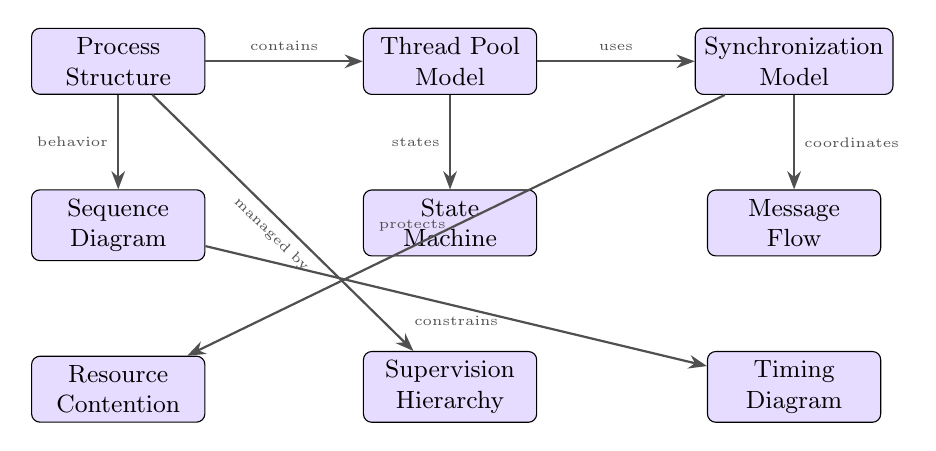
\begin{tikzpicture}[
    node distance=1.2cm and 2cm,
    model/.style={draw, fill=processcolor, rounded corners=3pt, minimum width=2.2cm, minimum height=0.7cm, font=\small, align=center},
    arrow/.style={-{Stealth}, thick, darkgray}
]
    % Nodes - top row
    \node[model] (process) {Process\\Structure};
    \node[model, right=2cm of process] (thread) {Thread Pool\\Model};
    \node[model, right=2cm of thread] (sync) {Synchronization\\Model};
    
    % Nodes - middle row
    \node[model, below=1.2cm of process] (sequence) {Sequence\\Diagram};
    \node[model, below=1.2cm of thread] (state) {State\\Machine};
    \node[model, below=1.2cm of sync] (message) {Message\\Flow};
    
    % Nodes - bottom row
    \node[model, below=1.2cm of sequence] (resource) {Resource\\Contention};
    \node[model, below=1.2cm of state] (supervision) {Supervision\\Hierarchy};
    \node[model, below=1.2cm of message] (timing) {Timing\\Diagram};
    
    % Arrows
    \draw[arrow] (process) -- (thread) node[midway, above, font=\tiny] {contains};
    \draw[arrow] (thread) -- (sync) node[midway, above, font=\tiny] {uses};
    \draw[arrow] (process) -- (sequence) node[midway, left, font=\tiny] {behavior};
    \draw[arrow] (thread) -- (state) node[midway, left, font=\tiny] {states};
    \draw[arrow] (sync) -- (message) node[midway, right, font=\tiny] {coordinates};
    \draw[arrow] (sync) -- (resource) node[midway, left, font=\tiny] {protects};
    \draw[arrow] (process) -- (supervision) node[midway, below, sloped, font=\tiny] {managed by};
    \draw[arrow] (sequence) -- (timing) node[midway, below, font=\tiny] {constrains};
\end{tikzpicture}
\caption{Model Type Dependency Relationships}
\end{figure}

% =============================================================================
% SECTION: MODEL LANGUAGES
% =============================================================================
\section{Model Languages}

For each model type, specific languages, notations, and techniques are prescribed.

\subsection{Process Diagram Notation}

\begin{figure}[H]
\centering
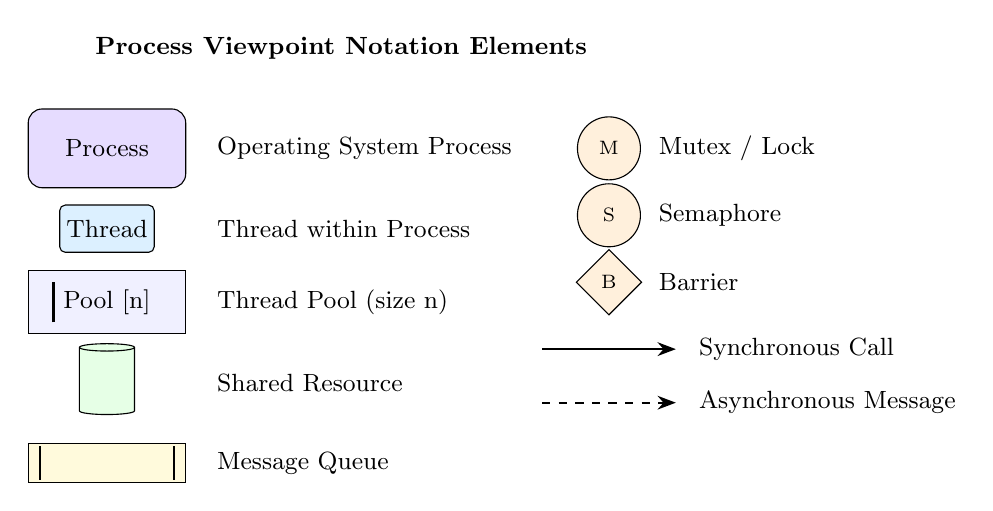
\begin{tikzpicture}[scale=0.85]
    % Legend title
    \node[font=\small\bfseries] at (0, 5) {Process Viewpoint Notation Elements};
    
    % Process
    \node[draw, fill=processcolor, rounded corners=5pt, minimum width=2cm, minimum height=1cm] at (-3.5, 3.5) {};
    \node[font=\small] at (-3.5, 3.5) {Process};
    \node[right, font=\small] at (-2, 3.5) {Operating System Process};
    
    % Thread
    \node[draw, fill=threadcolor, rounded corners=2pt, minimum width=1.2cm, minimum height=0.6cm] at (-3.5, 2.3) {};
    \node[font=\small] at (-3.5, 2.3) {Thread};
    \node[right, font=\small] at (-2, 2.3) {Thread within Process};
    
    % Thread Pool
    \node[draw, fill=poolcolor, minimum width=2cm, minimum height=0.8cm] at (-3.5, 1.2) {};
    \draw[thick] (-4.3, 0.9) -- (-4.3, 1.5);
    \node[font=\small] at (-3.5, 1.2) {Pool [n]};
    \node[right, font=\small] at (-2, 1.2) {Thread Pool (size n)};
    
    % Shared Resource
    \node[draw, fill=resourcecolor, cylinder, shape border rotate=90, aspect=0.4, minimum height=0.9cm, minimum width=0.7cm] at (-3.5, 0) {};
    \node[right, font=\small] at (-2, 0) {Shared Resource};
    
    % Synchronization primitives
    \node[draw, fill=synccolor, circle, minimum size=0.8cm, font=\scriptsize] at (4, 3.5) {M};
    \node[right, font=\small] at (4.6, 3.5) {Mutex / Lock};
    
    \node[draw, fill=synccolor, circle, minimum size=0.8cm, font=\scriptsize] at (4, 2.5) {S};
    \node[right, font=\small] at (4.6, 2.5) {Semaphore};
    
    \node[draw, fill=synccolor, diamond, minimum size=0.8cm, font=\scriptsize] at (4, 1.5) {B};
    \node[right, font=\small] at (4.6, 1.5) {Barrier};
    
    % Communication
    \draw[-{Stealth}, thick] (3, 0.5) -- (5, 0.5);
    \node[right, font=\small] at (5.2, 0.5) {Synchronous Call};
    
    \draw[-{Stealth}, thick, dashed] (3, -0.3) -- (5, -0.3);
    \node[right, font=\small] at (5.2, -0.3) {Asynchronous Message};
    
    % Queue
    \node[draw, fill=queuecolor, minimum width=2cm, minimum height=0.5cm] at (-3.5, -1.2) {};
    \draw[thick] (-4.5, -1.45) -- (-4.5, -0.95);
    \draw[thick] (-2.5, -1.45) -- (-2.5, -0.95);
    \node[right, font=\small] at (-2, -1.2) {Message Queue};
    
\end{tikzpicture}
\caption{Process Viewpoint Notation Legend}
\end{figure}

\subsection{Synchronization Primitive Summary}

\begin{table}[H]
\centering
\caption{Synchronization Primitive Comparison}
\small
\begin{tabular}{@{}L{2.2cm}L{3.5cm}L{4cm}L{3.5cm}@{}}
\toprule
\textbf{Primitive} & \textbf{Purpose} & \textbf{Operations} & \textbf{Use Cases} \\
\midrule
Mutex & Mutual exclusion & lock(), unlock() & Protecting critical sections \\
\addlinespace
Semaphore & Resource counting & wait(), signal() & Limiting concurrent access \\
\addlinespace
Condition Variable & Wait for condition & wait(), notify(), notifyAll() & Producer-consumer \\
\addlinespace
Read-Write Lock & Concurrent reads & readLock(), writeLock() & Read-heavy workloads \\
\addlinespace
Barrier & Synchronization point & await() & Phased computation \\
\addlinespace
Monitor & Encapsulated sync & synchronized methods & Object-level protection \\
\addlinespace
Channel & Message passing & send(), receive() & CSP-style concurrency \\
\addlinespace
Atomic Operations & Lock-free access & compareAndSwap() & High-performance counters \\
\bottomrule
\end{tabular}
\end{table}

\subsection{IPC Mechanism Comparison}

\begin{table}[H]
\centering
\caption{Inter-Process Communication Mechanisms}
\small
\begin{tabular}{@{}L{2.2cm}L{2cm}L{2cm}L{3cm}L{3.5cm}@{}}
\toprule
\textbf{Mechanism} & \textbf{Scope} & \textbf{Sync/Async} & \textbf{Data Copy} & \textbf{Use Cases} \\
\midrule
Shared Memory & Same machine & Async & Zero-copy & High throughput, low latency \\
\addlinespace
Pipes & Same machine & Sync/Async & Yes & Parent-child, streaming \\
\addlinespace
Message Queues & Same machine & Async & Yes & Decoupled producers/consumers \\
\addlinespace
Sockets & Network & Both & Yes & Distributed systems \\
\addlinespace
Signals & Same machine & Async & No data & Event notification \\
\addlinespace
Memory-mapped Files & Same machine & Async & Varies & Persistent shared state \\
\addlinespace
RPC/gRPC & Network & Sync & Serialized & Service communication \\
\bottomrule
\end{tabular}
\end{table}

\subsection{Threading Model Comparison}

\begin{table}[H]
\centering
\caption{Threading Model Comparison}
\small
\begin{tabular}{@{}L{2.5cm}L{4cm}L{3.5cm}L{3cm}@{}}
\toprule
\textbf{Model} & \textbf{Description} & \textbf{Advantages} & \textbf{Disadvantages} \\
\midrule
Thread-per-Request & New thread for each request & Simple model & High overhead at scale \\
\addlinespace
Thread Pool & Fixed pool processes tasks & Bounded resources & Queue management \\
\addlinespace
Event Loop & Single thread, async I/O & Low overhead, scalable & Blocking is problematic \\
\addlinespace
Actor Model & Isolated actors with mailboxes & No shared state & Message overhead \\
\addlinespace
Fork-Join & Recursive task splitting & Good for divide-conquer & Task granularity \\
\addlinespace
Work Stealing & Idle threads steal work & Load balancing & Complexity \\
\bottomrule
\end{tabular}
\end{table}

\subsection{Pseudocode Conventions}

\begin{lstlisting}[caption={Concurrency Pseudocode Example}, language=pseudocode]
// Process definition
process WebServer {
    thread pool workerPool[16]     // Thread pool with 16 workers
    channel<Request> requestQueue  // Bounded channel for requests
    mutex configLock               // Protects configuration state
    
    // Main thread - accepts connections
    while running {
        connection = accept()
        request = parseRequest(connection)
        requestQueue.send(request)  // Async send to queue
    }
}

// Worker thread definition
thread Worker {
    while running {
        request = requestQueue.receive()  // Blocks until message
        
        // Critical section - protected by lock
        synchronized(configLock) {
            config = readConfig()
        }
        
        response = processRequest(request, config)
        request.connection.send(response)
    }
}

// Parallel computation example
parallel for i in range(0, data.length) {
    results[i] = compute(data[i])
}
barrier.await()  // Wait for all iterations
aggregate(results)
\end{lstlisting}

\subsection{Tabular Specifications}

\subsubsection{Process Catalog Table}

\begin{table}[H]
\centering
\caption{Example Process Catalog Format}
\small
\begin{tabular}{@{}L{2cm}L{2.5cm}L{2cm}L{2.5cm}L{3.5cm}@{}}
\toprule
\textbf{Process} & \textbf{Role} & \textbf{Instances} & \textbf{Lifecycle} & \textbf{Communication} \\
\midrule
API Gateway & Request routing & 3 (HA) & Long-running & HTTP in, gRPC out \\
Order Service & Order processing & 5 (scaled) & Long-running & gRPC, Kafka \\
Worker & Background tasks & Auto-scaled & Transient & Redis queue \\
Scheduler & Task scheduling & 1 (singleton) & Long-running & Database, Redis \\
\bottomrule
\end{tabular}
\end{table}

\subsubsection{Thread Pool Configuration Table}

\begin{table}[H]
\centering
\caption{Example Thread Pool Configuration}
\small
\begin{tabular}{@{}L{2.5cm}L{1.5cm}L{1.5cm}L{2cm}L{2cm}L{3cm}@{}}
\toprule
\textbf{Pool Name} & \textbf{Core} & \textbf{Max} & \textbf{Queue} & \textbf{Timeout} & \textbf{Purpose} \\
\midrule
http-workers & 10 & 100 & Unbounded & 30s & HTTP request handling \\
db-pool & 20 & 20 & Bounded(50) & 10s & Database operations \\
async-io & 4 & 4 & Unbounded & -- & Async I/O completion \\
scheduled & 2 & 10 & Delayed & -- & Scheduled tasks \\
\bottomrule
\end{tabular}
\end{table}

\subsubsection{Lock Inventory Table}

\begin{table}[H]
\centering
\caption{Example Lock Inventory}
\small
\begin{tabular}{@{}L{2.5cm}L{2cm}L{3cm}L{2.5cm}L{2.5cm}@{}}
\toprule
\textbf{Lock Name} & \textbf{Type} & \textbf{Protects} & \textbf{Contention} & \textbf{Order} \\
\midrule
configLock & RWLock & Configuration state & Low (mostly reads) & 1 \\
cacheLock & Mutex & Cache structure & Medium & 2 \\
sessionLock[id] & Mutex & Per-session state & Low (partitioned) & 3 \\
globalStats & Atomic & Statistics counters & High (lock-free) & -- \\
\bottomrule
\end{tabular}
\end{table}

% =============================================================================
% SECTION: VIEWPOINT METAMODELS
% =============================================================================
\section{Viewpoint Metamodels}

This section defines the conceptual metamodel underlying the Process Viewpoint.

\subsection{Core Metamodel}

\begin{figure}[H]
\centering
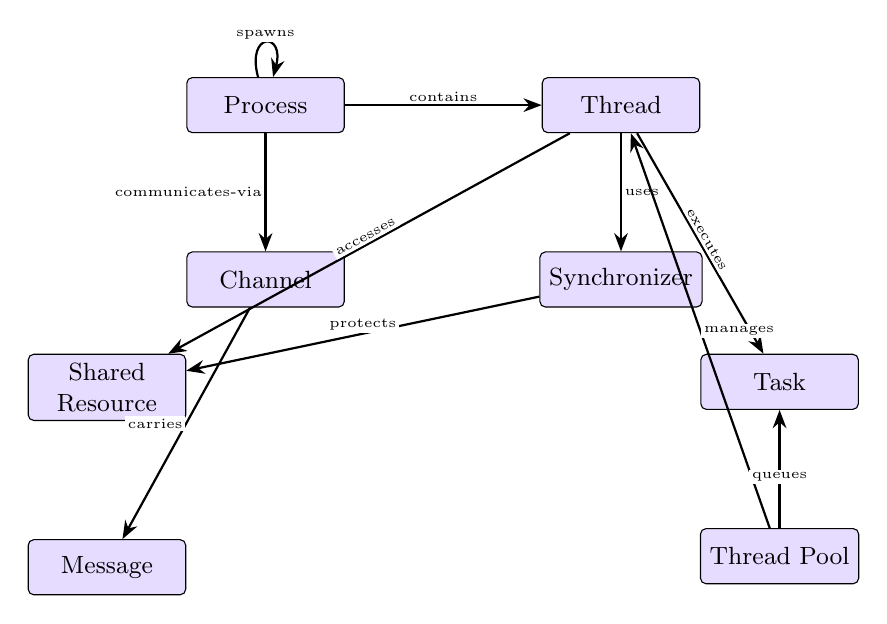
\begin{tikzpicture}[
    node distance=1.3cm and 2cm,
    entity/.style={draw, fill=processcolor, rounded corners=2pt, minimum width=2cm, minimum height=0.7cm, font=\small, align=center},
    arrow/.style={-{Stealth}, thick},
    label/.style={font=\tiny, fill=white, inner sep=1pt}
]
    % Main entities
    \node[entity] (process) {Process};
    \node[entity, right=2.5cm of process] (thread) {Thread};
    \node[entity, below=1.5cm of process] (channel) {Channel};
    \node[entity, below=1.5cm of thread] (sync) {Synchronizer};
    \node[entity, below left=2.8cm and 0cm of process] (resource) {Shared\\Resource};
    \node[entity, below right=2.8cm and 0cm of thread] (task) {Task};
    \node[entity, below=1.5cm of resource] (message) {Message};
    \node[entity, below=1.5cm of task] (pool) {Thread Pool};
    
    % Relationships
    \draw[arrow] (process) -- (thread) node[label, midway, above] {contains};
    \draw[arrow] (process) -- (channel) node[label, midway, left] {communicates-via};
    \draw[arrow] (thread) -- (sync) node[label, midway, right] {uses};
    \draw[arrow] (thread) -- (resource) node[label, midway, above, sloped] {accesses};
    \draw[arrow] (sync) -- (resource) node[label, midway, above] {protects};
    \draw[arrow] (thread) -- (task) node[label, midway, above, sloped] {executes};
    \draw[arrow] (channel) -- (message) node[label, midway, left] {carries};
    \draw[arrow] (pool) -- (thread) node[label, midway, right] {manages};
    \draw[arrow] (pool) -- (task) node[label, midway, below] {queues};
    
    % Self-reference
    \draw[arrow] (process) to[loop above] node[label, above] {spawns} (process);
\end{tikzpicture}
\caption{Process Viewpoint Core Metamodel}
\end{figure}

\subsection{Entity Definitions}

\begin{definitionbox}[Entity: Process]
\textbf{Definition:} An operating system process that provides an isolated execution environment with its own address space, resources, and one or more threads of execution.

\textbf{Attributes:}
\begin{itemize}[nosep]
    \item \texttt{processId}: Unique identifier
    \item \texttt{name}: Process name
    \item \texttt{description}: Purpose of the process
    \item \texttt{executable}: Binary or script that runs
    \item \texttt{instances}: Number of instances (1, N, auto-scaled)
    \item \texttt{lifecycle}: Lifecycle type (long-running, transient, scheduled)
    \item \texttt{priority}: Scheduling priority
    \item \texttt{resourceLimits}: CPU, memory, file descriptor limits
    \item \texttt{restartPolicy}: What happens on failure
    \item \texttt{dependencies}: Other processes this depends on
    \item \texttt{healthCheck}: How health is determined
\end{itemize}

\textbf{Constraints:}
\begin{itemize}[nosep]
    \item Every process must have at least one thread
    \item Long-running processes must have health checks
    \item Resource limits must be specified for production
    \item Restart policies must be defined
\end{itemize}
\end{definitionbox}

\begin{definitionbox}[Entity: Thread]
\textbf{Definition:} A unit of execution within a process that shares the process's address space but has its own stack, program counter, and thread-local storage.

\textbf{Attributes:}
\begin{itemize}[nosep]
    \item \texttt{threadId}: Unique identifier within process
    \item \texttt{name}: Thread name (for debugging)
    \item \texttt{type}: Thread type (main, worker, I/O, timer, daemon)
    \item \texttt{priority}: Thread priority
    \item \texttt{stackSize}: Stack size allocation
    \item \texttt{state}: Current state (new, runnable, blocked, waiting, terminated)
    \item \texttt{cpuAffinity}: CPU cores thread can run on
    \item \texttt{daemon}: Whether thread prevents process exit
    \item \texttt{interruptible}: Whether thread can be interrupted
\end{itemize}

\textbf{Constraints:}
\begin{itemize}[nosep]
    \item Daemon threads should not hold critical resources
    \item Thread names should be meaningful for debugging
    \item Stack size should be appropriate for workload
\end{itemize}
\end{definitionbox}

\begin{definitionbox}[Entity: Thread Pool]
\textbf{Definition:} A managed collection of pre-created threads that execute submitted tasks, providing efficient thread reuse and bounded concurrency.

\textbf{Attributes:}
\begin{itemize}[nosep]
    \item \texttt{poolId}: Unique identifier
    \item \texttt{name}: Pool name
    \item \texttt{coreSize}: Minimum number of threads maintained
    \item \texttt{maxSize}: Maximum number of threads allowed
    \item \texttt{queueType}: Type of task queue (bounded, unbounded, synchronous)
    \item \texttt{queueCapacity}: Maximum queue size (if bounded)
    \item \texttt{keepAliveTime}: How long idle threads are kept
    \item \texttt{rejectionPolicy}: What happens when pool is full
    \item \texttt{threadFactory}: How threads are created
    \item \texttt{metrics}: Pool utilization metrics
\end{itemize}

\textbf{Constraints:}
\begin{itemize}[nosep]
    \item Core size $\leq$ max size
    \item Rejection policy must be defined for bounded queues
    \item Pool sizing should be based on workload analysis
    \item Metrics should be exposed for monitoring
\end{itemize}
\end{definitionbox}

\begin{definitionbox}[Entity: Synchronizer]
\textbf{Definition:} A concurrency control mechanism that coordinates access to shared resources or synchronizes execution between threads.

\textbf{Attributes:}
\begin{itemize}[nosep]
    \item \texttt{synchronizerId}: Unique identifier
    \item \texttt{name}: Synchronizer name
    \item \texttt{type}: Type (mutex, semaphore, rwlock, barrier, condition, monitor)
    \item \texttt{fairness}: Whether waiting threads are served in order
    \item \texttt{permits}: Number of permits (for semaphores)
    \item \texttt{reentrant}: Whether same thread can acquire multiple times
    \item \texttt{timeout}: Default timeout for acquisition
    \item \texttt{owner}: Current owner (for mutexes)
    \item \texttt{waiters}: Number of waiting threads
\end{itemize}

\textbf{Constraints:}
\begin{itemize}[nosep]
    \item Locks must be released in reverse order of acquisition
    \item Timeouts should be used to prevent indefinite blocking
    \item Lock ordering must be documented to prevent deadlock
\end{itemize}
\end{definitionbox}

\begin{definitionbox}[Entity: Channel]
\textbf{Definition:} A communication pathway between processes or threads for exchanging messages, providing decoupled, type-safe communication.

\textbf{Attributes:}
\begin{itemize}[nosep]
    \item \texttt{channelId}: Unique identifier
    \item \texttt{name}: Channel name
    \item \texttt{type}: Channel type (unbuffered, buffered, broadcast)
    \item \texttt{capacity}: Buffer capacity (for buffered channels)
    \item \texttt{messageType}: Type of messages carried
    \item \texttt{producers}: Processes/threads that send
    \item \texttt{consumers}: Processes/threads that receive
    \item \texttt{deliveryGuarantee}: At-most-once, at-least-once, exactly-once
    \item \texttt{ordering}: FIFO, priority, unordered
\end{itemize}

\textbf{Constraints:}
\begin{itemize}[nosep]
    \item Unbuffered channels block sender until receiver ready
    \item Buffer capacity should be sized based on load analysis
    \item Message types should be well-defined
\end{itemize}
\end{definitionbox}

\begin{definitionbox}[Entity: Shared Resource]
\textbf{Definition:} A system resource (memory, file, connection, etc.) that is accessed by multiple threads or processes and requires coordination.

\textbf{Attributes:}
\begin{itemize}[nosep]
    \item \texttt{resourceId}: Unique identifier
    \item \texttt{name}: Resource name
    \item \texttt{type}: Resource type (memory, file, connection, device)
    \item \texttt{accessMode}: How resource can be accessed (read, write, exclusive)
    \item \texttt{capacity}: Resource capacity or limit
    \item \texttt{protection}: Synchronization mechanism protecting it
    \item \texttt{consumers}: Threads/processes that access it
    \item \texttt{contentionLevel}: Expected contention (low, medium, high)
\end{itemize}

\textbf{Constraints:}
\begin{itemize}[nosep]
    \item All shared mutable resources must have protection
    \item High-contention resources should use appropriate techniques
    \item Resource access patterns should be documented
\end{itemize}
\end{definitionbox}

\begin{definitionbox}[Entity: Task]
\textbf{Definition:} A unit of work that can be submitted for execution by a thread, representing a discrete computation or operation.

\textbf{Attributes:}
\begin{itemize}[nosep]
    \item \texttt{taskId}: Unique identifier
    \item \texttt{name}: Task name or type
    \item \texttt{priority}: Execution priority
    \item \texttt{state}: Current state (pending, running, completed, failed, cancelled)
    \item \texttt{timeout}: Maximum execution time
    \item \texttt{retryPolicy}: How failures are retried
    \item \texttt{dependencies}: Other tasks this depends on
    \item \texttt{result}: Result or error from execution
    \item \texttt{cancellable}: Whether task can be cancelled
\end{itemize}

\textbf{Constraints:}
\begin{itemize}[nosep]
    \item Tasks should be designed for cancellation
    \item Long-running tasks should support progress reporting
    \item Task dependencies must be acyclic
\end{itemize}
\end{definitionbox}

\begin{definitionbox}[Entity: Message]
\textbf{Definition:} A unit of data transmitted between processes or threads through a communication channel.

\textbf{Attributes:}
\begin{itemize}[nosep]
    \item \texttt{messageId}: Unique identifier
    \item \texttt{type}: Message type or schema
    \item \texttt{payload}: Message content
    \item \texttt{sender}: Sending process/thread
    \item \texttt{recipient}: Receiving process/thread (if point-to-point)
    \item \texttt{timestamp}: When message was created
    \item \texttt{correlationId}: For request-response correlation
    \item \texttt{priority}: Message priority
    \item \texttt{ttl}: Time-to-live before expiration
\end{itemize}

\textbf{Constraints:}
\begin{itemize}[nosep]
    \item Messages should be immutable after creation
    \item Message types should be versioned for compatibility
    \item Large messages should be chunked or use references
\end{itemize}
\end{definitionbox}

\subsection{Relationship Definitions}

\begin{table}[H]
\centering
\caption{Metamodel Relationship Definitions}
\small
\begin{tabular}{@{}L{2.3cm}L{1.8cm}L{1.8cm}L{7.5cm}@{}}
\toprule
\textbf{Relationship} & \textbf{Source} & \textbf{Target} & \textbf{Description} \\
\midrule
contains & Process & Thread & Process has this thread \\
\addlinespace
spawns & Process & Process & Process creates child process \\
\addlinespace
communicates-via & Process & Channel & Process uses channel for IPC \\
\addlinespace
uses & Thread & Synchronizer & Thread uses this sync primitive \\
\addlinespace
accesses & Thread & Resource & Thread reads/writes resource \\
\addlinespace
protects & Synchronizer & Resource & Synchronizer guards resource \\
\addlinespace
executes & Thread & Task & Thread runs this task \\
\addlinespace
manages & Pool & Thread & Pool controls thread lifecycle \\
\addlinespace
queues & Pool & Task & Pool holds pending tasks \\
\addlinespace
carries & Channel & Message & Channel transmits messages \\
\bottomrule
\end{tabular}
\end{table}

% =============================================================================
% SECTION: CONFORMING NOTATIONS
% =============================================================================
\section{Conforming Notations}

Several existing notations and modeling approaches align with the Process Viewpoint.

\subsection{UML Behavioral Diagrams}

UML provides several diagram types suitable for modeling concurrent behavior:

\textbf{Activity Diagrams:} Fork/join nodes for parallelism, swimlanes for process assignment.

\textbf{Sequence Diagrams:} Par/alt combined fragments for concurrent messaging.

\textbf{State Machine Diagrams:} Orthogonal regions for concurrent states.

\textbf{Conformance Level:} Full support for concurrency modeling with appropriate extensions.

\subsection{Petri Nets}

Petri nets provide formal modeling of concurrent systems with mathematical analysis capabilities.

\textbf{Elements:} Places (states), transitions (events), tokens (resources/control).

\textbf{Analysis:} Reachability, boundedness, liveness, deadlock detection.

\textbf{Conformance Level:} Strong for formal analysis, less intuitive for communication.

\subsection{CSP (Communicating Sequential Processes)}

CSP provides algebraic notation for describing concurrent process interaction.

\textbf{Operators:} Sequential composition, parallel composition, choice, interleaving.

\textbf{Tools:} FDR model checker for refinement checking.

\textbf{Conformance Level:} Excellent for formal specification and verification.

\subsection{Process Algebra Comparison}

\begin{table}[H]
\centering
\caption{Process Algebra and Formal Method Comparison}
\small
\begin{tabular}{@{}L{2.5cm}L{3.5cm}L{3.5cm}L{3.5cm}@{}}
\toprule
\textbf{Approach} & \textbf{Strengths} & \textbf{Tool Support} & \textbf{Best For} \\
\midrule
CSP & Communication focus & FDR, PAT & Message-passing systems \\
\addlinespace
CCS & Bisimulation theory & CWB, mCRL2 & Mobile/dynamic systems \\
\addlinespace
Petri Nets & Visual, analyzable & PIPE, CPN Tools & Resource/workflow modeling \\
\addlinespace
TLA+ & State-based, practical & TLC model checker & Distributed algorithms \\
\addlinespace
Promela/SPIN & Model checking & SPIN & Protocol verification \\
\bottomrule
\end{tabular}
\end{table}

% =============================================================================
% SECTION: MODEL CORRESPONDENCE RULES
% =============================================================================
\section{Model Correspondence Rules}

Model correspondence rules define how elements in process models relate to elements in other architectural views.

\subsection{Deployment View Correspondence}

\begin{definitionbox}[Correspondence Rule CR-01: Process to Node Mapping]
\textbf{Rule:} Every process must be allocated to at least one deployment node.

\textbf{Formal Expression:}
\begin{center}
$\forall p \in Processes : \exists N \subseteq Nodes : executes\_on(p, N)$
\end{center}

\textbf{Rationale:} Ensures all processes have defined execution location.

\textbf{Verification:} Deployment manifest review.
\end{definitionbox}

\begin{definitionbox}[Correspondence Rule CR-02: Thread Pool to Resources]
\textbf{Rule:} Thread pool sizing must be compatible with deployment node resources.

\textbf{Formal Expression:}
\begin{center}
$\forall pool \in ThreadPools, node \in Nodes : pool.maxSize \leq node.cores \times factor$
\end{center}

\textbf{Rationale:} Prevents over-subscription of CPU resources.

\textbf{Verification:} Capacity analysis.
\end{definitionbox}

\subsection{Development View Correspondence}

\begin{definitionbox}[Correspondence Rule CR-03: Thread to Module Mapping]
\textbf{Rule:} Thread implementations must trace to code modules.

\textbf{Formal Expression:}
\begin{center}
$\forall t \in Threads : \exists m \in Modules : implements(m, t)$
\end{center}

\textbf{Rationale:} Ensures thread designs are implemented in code.

\textbf{Verification:} Code review, traceability matrix.
\end{definitionbox}

\subsection{Component-and-Connector View Correspondence}

\begin{definitionbox}[Correspondence Rule CR-04: Channel to Connector Mapping]
\textbf{Rule:} Inter-process channels must correspond to C\&C connectors.

\textbf{Formal Expression:}
\begin{center}
$\forall ch \in Channels_{IPC} : \exists conn \in Connectors : realizes(conn, ch)$
\end{center}

\textbf{Rationale:} Ensures IPC mechanisms are architecturally visible.

\textbf{Verification:} Architecture diagram comparison.
\end{definitionbox}

% =============================================================================
% SECTION: OPERATIONS ON VIEWS
% =============================================================================
\section{Operations on Views}

This section defines methods for creating, interpreting, analyzing, and implementing process views.

\subsection{Creation Methods}

\subsubsection{View Development Process}

\begin{guidancebox}[Step 1: Identify Execution Requirements]
\begin{enumerate}[nosep]
    \item Gather performance and scalability requirements
    \item Identify real-time or latency constraints
    \item Determine throughput requirements
    \item Assess resource constraints (CPU, memory)
    \item Review reliability and availability requirements
\end{enumerate}
\end{guidancebox}

\begin{guidancebox}[Step 2: Define Process Structure]
\begin{enumerate}[nosep]
    \item Identify major system processes
    \item Determine process boundaries based on isolation needs
    \item Define process lifecycle (long-running, transient, scheduled)
    \item Specify process instances and scaling strategy
    \item Document process dependencies and startup order
\end{enumerate}
\end{guidancebox}

\begin{guidancebox}[Step 3: Design Thread Architecture]
\begin{enumerate}[nosep]
    \item Choose threading model (thread-per-request, pool, event loop)
    \item Size thread pools based on workload analysis
    \item Identify CPU-bound vs I/O-bound workloads
    \item Define thread types and responsibilities
    \item Plan thread-local storage needs
\end{enumerate}
\end{guidancebox}

\begin{guidancebox}[Step 4: Identify Shared Resources]
\begin{enumerate}[nosep]
    \item Enumerate shared mutable state
    \item Classify access patterns (read-heavy, write-heavy, balanced)
    \item Assess contention levels
    \item Identify immutable vs mutable data
    \item Consider partitioning strategies
\end{enumerate}
\end{guidancebox}

\begin{guidancebox}[Step 5: Design Synchronization Strategy]
\begin{enumerate}[nosep]
    \item Select appropriate synchronization primitives
    \item Define lock ordering to prevent deadlock
    \item Minimize lock scope and duration
    \item Consider lock-free alternatives for hot paths
    \item Document critical sections
\end{enumerate}
\end{guidancebox}

\begin{guidancebox}[Step 6: Define Communication Patterns]
\begin{enumerate}[nosep]
    \item Choose IPC mechanisms based on requirements
    \item Define message formats and protocols
    \item Specify synchronous vs asynchronous communication
    \item Plan for communication failures
    \item Document channel capacities and backpressure
\end{enumerate}
\end{guidancebox}

\begin{guidancebox}[Step 7: Validate and Analyze]
\begin{enumerate}[nosep]
    \item Review for deadlock potential
    \item Analyze for race conditions
    \item Verify resource bounds
    \item Test under load conditions
    \item Document known concurrency hazards
\end{enumerate}
\end{guidancebox}

\subsubsection{Common Concurrency Patterns}

\begin{patternbox}[Pattern: Producer-Consumer]
\textbf{Context:} Decouple data production from consumption with different rates.

\textbf{Solution:} Use bounded queue between producer and consumer threads.

\textbf{Elements:}
\begin{itemize}[nosep]
    \item Producer thread(s) add items to queue
    \item Consumer thread(s) remove items from queue
    \item Queue provides buffering and synchronization
    \item Backpressure when queue is full
\end{itemize}

\textbf{Use When:} Rate mismatch between stages, decoupling needed.
\end{patternbox}

\begin{patternbox}[Pattern: Worker Pool]
\textbf{Context:} Process many independent tasks efficiently.

\textbf{Solution:} Fixed pool of worker threads processing task queue.

\textbf{Elements:}
\begin{itemize}[nosep]
    \item Task queue holds pending work
    \item Worker threads pull tasks from queue
    \item Pool manager handles thread lifecycle
    \item Rejection policy for queue overflow
\end{itemize}

\textbf{Use When:} Many independent tasks, bounded resource usage needed.
\end{patternbox}

\begin{patternbox}[Pattern: Read-Write Lock]
\textbf{Context:} Resource with many readers, few writers.

\textbf{Solution:} Allow concurrent reads, exclusive writes.

\textbf{Elements:}
\begin{itemize}[nosep]
    \item Multiple readers can hold read lock simultaneously
    \item Writer requires exclusive access (no readers or writers)
    \item Typically writer preference to prevent starvation
\end{itemize}

\textbf{Use When:} Read-heavy workloads, shared data structures.
\end{patternbox}

\begin{patternbox}[Pattern: Actor Model]
\textbf{Context:} Avoid shared mutable state entirely.

\textbf{Solution:} Isolated actors communicate only via messages.

\textbf{Elements:}
\begin{itemize}[nosep]
    \item Actors encapsulate state and behavior
    \item Communication via asynchronous messages
    \item Each actor processes one message at a time
    \item Supervision hierarchies for fault tolerance
\end{itemize}

\textbf{Use When:} Complex concurrency, fault tolerance critical.
\end{patternbox}

\begin{patternbox}[Pattern: Future/Promise]
\textbf{Context:} Asynchronous operations with eventual results.

\textbf{Solution:} Placeholder for result that will be available later.

\textbf{Elements:}
\begin{itemize}[nosep]
    \item Future represents pending computation result
    \item Promise allows setting the result
    \item Callbacks or blocking wait for completion
    \item Composition of multiple futures
\end{itemize}

\textbf{Use When:} Async operations, non-blocking code, composition.
\end{patternbox}

\begin{table}[H]
\centering
\caption{Concurrency Patterns Summary}
\small
\begin{tabular}{@{}L{2.8cm}L{4.2cm}L{5.5cm}@{}}
\toprule
\textbf{Pattern} & \textbf{Description} & \textbf{Use When} \\
\midrule
Producer-Consumer & Queue between producer/consumer & Rate decoupling, buffering \\
\addlinespace
Worker Pool & Fixed workers process task queue & Many independent tasks \\
\addlinespace
Read-Write Lock & Concurrent reads, exclusive writes & Read-heavy workloads \\
\addlinespace
Actor Model & Isolated actors, message passing & No shared state desired \\
\addlinespace
Future/Promise & Placeholder for async result & Async composition \\
\addlinespace
Barrier & Synchronization point & Phased computation \\
\addlinespace
Pipeline & Stages process in sequence & Stream processing \\
\addlinespace
Fork-Join & Recursive divide and conquer & Parallel algorithms \\
\addlinespace
Double-Checked Locking & Lazy init optimization & Singleton, lazy loading \\
\addlinespace
Thread-Local Storage & Per-thread state & Avoid sharing, context \\
\bottomrule
\end{tabular}
\end{table}

\subsection{Analysis Methods}

\subsubsection{Deadlock Analysis}

\begin{hazardbox}[Deadlock Detection Checklist]
\textbf{Four Necessary Conditions for Deadlock:}
\begin{enumerate}[nosep]
    \item \textbf{Mutual Exclusion:} Resources held exclusively
    \item \textbf{Hold and Wait:} Holding resources while waiting for more
    \item \textbf{No Preemption:} Resources cannot be forcibly taken
    \item \textbf{Circular Wait:} Circular chain of waiting
\end{enumerate}

\textbf{Prevention Strategies:}
\begin{itemize}[nosep]
    \item Establish and enforce lock ordering
    \item Use timeout-based lock acquisition
    \item Acquire all locks atomically
    \item Use lock-free data structures where possible
\end{itemize}
\end{hazardbox}

\subsubsection{Race Condition Analysis}

\begin{hazardbox}[Race Condition Identification]
\textbf{Check for races when:}
\begin{itemize}[nosep]
    \item Multiple threads access shared mutable state
    \item At least one access is a write
    \item Accesses are not synchronized
    \item Order of operations affects outcome
\end{itemize}

\textbf{Common Race Condition Types:}
\begin{itemize}[nosep]
    \item Check-then-act (TOCTOU)
    \item Read-modify-write without atomicity
    \item Lazy initialization races
    \item Publication of partially constructed objects
\end{itemize}
\end{hazardbox}

\subsubsection{Performance Analysis}

\begin{definitionbox}[Amdahl's Law]
\textbf{Purpose:} Calculate theoretical speedup from parallelization.

\textbf{Formula:}
\begin{center}
$Speedup = \frac{1}{(1-P) + \frac{P}{N}}$
\end{center}

Where:
\begin{itemize}[nosep]
    \item $P$ = Proportion of program that can be parallelized
    \item $N$ = Number of processors
    \item $(1-P)$ = Sequential portion (limits speedup)
\end{itemize}

\textbf{Implications:}
\begin{itemize}[nosep]
    \item Even small sequential portions limit scalability
    \item Focus optimization on sequential bottlenecks
    \item Beyond certain $N$, adding processors has diminishing returns
\end{itemize}
\end{definitionbox}

\begin{definitionbox}[Little's Law]
\textbf{Purpose:} Relate throughput, latency, and concurrency.

\textbf{Formula:}
\begin{center}
$L = \lambda \times W$
\end{center}

Where:
\begin{itemize}[nosep]
    \item $L$ = Average number of items in system (concurrency)
    \item $\lambda$ = Average arrival rate (throughput)
    \item $W$ = Average time in system (latency)
\end{itemize}

\textbf{Application:}
\begin{itemize}[nosep]
    \item Size thread pools based on expected concurrency
    \item Predict queue lengths from arrival rates
    \item Balance throughput and latency goals
\end{itemize}
\end{definitionbox}

% =============================================================================
% SECTION: EXAMPLES
% =============================================================================
\section{Examples}

\subsection{Example 1: Web Application Process Architecture}

\begin{figure}[H]
\centering
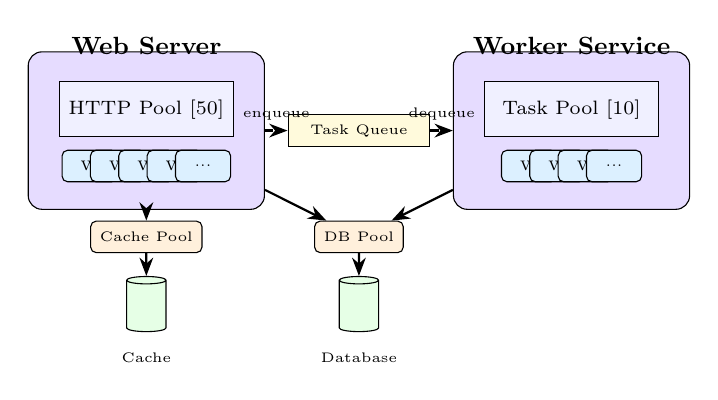
\begin{tikzpicture}[
    process/.style={draw, fill=processcolor, rounded corners=5pt, minimum width=3cm, minimum height=2cm},
    thread/.style={draw, fill=threadcolor, rounded corners=2pt, minimum width=0.7cm, minimum height=0.4cm, font=\tiny},
    pool/.style={draw, fill=poolcolor, minimum width=2.2cm, minimum height=0.7cm, font=\scriptsize},
    queue/.style={draw, fill=queuecolor, minimum width=1.8cm, minimum height=0.4cm, font=\tiny},
    resource/.style={draw, fill=resourcecolor, cylinder, shape border rotate=90, aspect=0.4, minimum height=0.7cm, minimum width=0.5cm, font=\tiny},
    scale=0.9
]
    % Web Server Process
    \node[process] (web) at (-3, 2) {};
    \node[font=\small\bfseries] at (-3, 3.2) {Web Server};
    \node[pool] at (-3, 2.3) {HTTP Pool [50]};
    \node[thread] at (-3.8, 1.5) {W};
    \node[thread] at (-3.4, 1.5) {W};
    \node[thread] at (-3, 1.5) {W};
    \node[thread] at (-2.6, 1.5) {W};
    \node[thread] at (-2.2, 1.5) {...};
    
    % Worker Process
    \node[process] (worker) at (3, 2) {};
    \node[font=\small\bfseries] at (3, 3.2) {Worker Service};
    \node[pool] at (3, 2.3) {Task Pool [10]};
    \node[thread] at (2.4, 1.5) {W};
    \node[thread] at (2.8, 1.5) {W};
    \node[thread] at (3.2, 1.5) {W};
    \node[thread] at (3.6, 1.5) {...};
    
    % Message Queue
    \node[queue] (mq) at (0, 2) {Task Queue};
    
    % Database
    \node[resource] (db) at (0, -0.5) {};
    \node[font=\tiny, below] at (0, -1) {Database};
    
    % Cache
    \node[resource] (cache) at (-3, -0.5) {};
    \node[font=\tiny, below] at (-3, -1) {Cache};
    
    % Connection pools
    \node[draw, fill=synccolor, rounded corners=2pt, minimum width=1cm, minimum height=0.4cm, font=\tiny] (dbpool) at (0, 0.5) {DB Pool};
    \node[draw, fill=synccolor, rounded corners=2pt, minimum width=1cm, minimum height=0.4cm, font=\tiny] (cachepool) at (-3, 0.5) {Cache Pool};
    
    % Connections
    \draw[-{Stealth}, thick, dashed] (web) -- (mq) node[midway, above, font=\tiny] {enqueue};
    \draw[-{Stealth}, thick, dashed] (mq) -- (worker) node[midway, above, font=\tiny] {dequeue};
    \draw[-{Stealth}, thick] (web) -- (cachepool);
    \draw[-{Stealth}, thick] (cachepool) -- (cache);
    \draw[-{Stealth}, thick] (web) -- (dbpool);
    \draw[-{Stealth}, thick] (worker) -- (dbpool);
    \draw[-{Stealth}, thick] (dbpool) -- (db);
    
\end{tikzpicture}
\caption{Web Application Process Architecture}
\end{figure}

\textbf{Description:} This diagram shows a typical web application with a multi-threaded web server process using a thread pool for handling HTTP requests. Background tasks are delegated via a message queue to a separate worker process with its own thread pool. Both processes share access to a database through a connection pool, and the web server uses a cache with its own pool.

\subsection{Example 2: Supervision Hierarchy}

\begin{figure}[H]
\centering
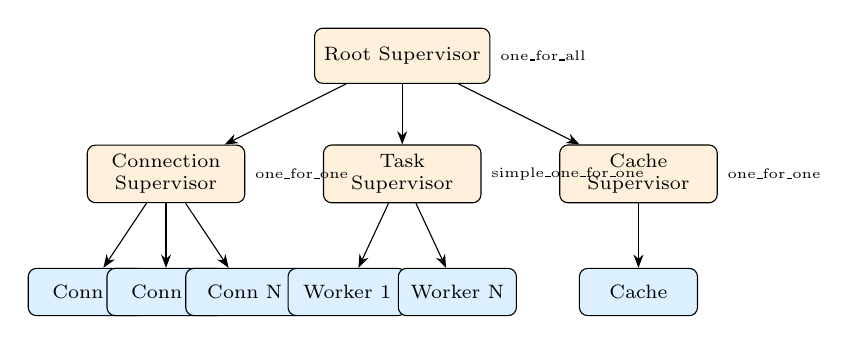
\begin{tikzpicture}[
    supervisor/.style={draw, fill=synccolor, rounded corners=3pt, minimum width=2cm, minimum height=0.7cm, font=\scriptsize},
    worker/.style={draw, fill=threadcolor, rounded corners=3pt, minimum width=1.5cm, minimum height=0.6cm, font=\scriptsize},
    level distance=1.5cm,
    sibling distance=2.5cm
]
    % Root supervisor
    \node[supervisor] (root) at (0, 3) {Root Supervisor};
    
    % Second level
    \node[supervisor, align=center] (conn) at (-3, 1.5) {Connection\\Supervisor};
    \node[supervisor, align=center] (task) at (0, 1.5) {Task\\Supervisor};
    \node[supervisor, align=center] (cache) at (3, 1.5) {Cache\\Supervisor};
    
    % Workers
    \node[worker] (c1) at (-4, 0) {Conn 1};
    \node[worker] (c2) at (-3, 0) {Conn 2};
    \node[worker] (c3) at (-2, 0) {Conn N};
    
    \node[worker] (t1) at (-0.7, 0) {Worker 1};
    \node[worker] (t2) at (0.7, 0) {Worker N};
    
    \node[worker] (ch1) at (3, 0) {Cache};
    
    % Connections
    \draw[-{Stealth}] (root) -- (conn);
    \draw[-{Stealth}] (root) -- (task);
    \draw[-{Stealth}] (root) -- (cache);
    
    \draw[-{Stealth}] (conn) -- (c1);
    \draw[-{Stealth}] (conn) -- (c2);
    \draw[-{Stealth}] (conn) -- (c3);
    
    \draw[-{Stealth}] (task) -- (t1);
    \draw[-{Stealth}] (task) -- (t2);
    
    \draw[-{Stealth}] (cache) -- (ch1);
    
    % Restart strategies
    \node[font=\tiny, right] at (root.east) {one\_for\_all};
    \node[font=\tiny, right] at (conn.east) {one\_for\_one};
    \node[font=\tiny, right] at (task.east) {simple\_one\_for\_one};
    \node[font=\tiny, right] at (cache.east) {one\_for\_one};
    
\end{tikzpicture}
\caption{Erlang/OTP-Style Supervision Hierarchy}
\end{figure}

\textbf{Description:} This supervision tree shows how processes are organized for fault tolerance. The root supervisor manages three child supervisors with different restart strategies. If any component fails, its supervisor can restart it without affecting unrelated parts of the system.

\subsection{Example 3: Lock Ordering Diagram}

\begin{figure}[H]
\centering
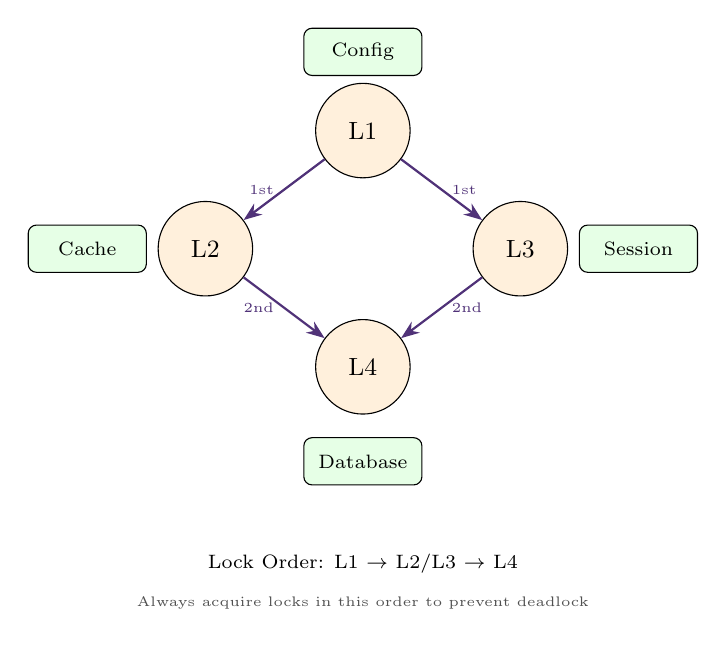
\begin{tikzpicture}[
    lock/.style={draw, fill=synccolor, circle, minimum size=1.2cm, font=\small},
    resource/.style={draw, fill=resourcecolor, rounded corners=3pt, minimum width=1.5cm, minimum height=0.6cm, font=\scriptsize}
]
    % Locks with ordering numbers
    \node[lock] (l1) at (0, 3) {L1};
    \node[lock] (l2) at (-2, 1.5) {L2};
    \node[lock] (l3) at (2, 1.5) {L3};
    \node[lock] (l4) at (0, 0) {L4};
    
    % Ordering arrows (acquire in this order)
    \draw[-{Stealth}, thick, primary] (l1) -- (l2) node[midway, left, font=\tiny] {1st};
    \draw[-{Stealth}, thick, primary] (l1) -- (l3) node[midway, right, font=\tiny] {1st};
    \draw[-{Stealth}, thick, primary] (l2) -- (l4) node[midway, left, font=\tiny] {2nd};
    \draw[-{Stealth}, thick, primary] (l3) -- (l4) node[midway, right, font=\tiny] {2nd};
    
    % Resources protected
    \node[resource] at (0, 4) {Config};
    \node[resource] at (-3.5, 1.5) {Cache};
    \node[resource] at (3.5, 1.5) {Session};
    \node[resource] at (0, -1.2) {Database};
    
    % Legend
    \node[font=\scriptsize] at (0, -2.5) {Lock Order: L1 $\rightarrow$ L2/L3 $\rightarrow$ L4};
    \node[font=\tiny, darkgray] at (0, -3) {Always acquire locks in this order to prevent deadlock};
    
\end{tikzpicture}
\caption{Lock Ordering to Prevent Deadlock}
\end{figure}

\textbf{Description:} This diagram shows the required lock acquisition order to prevent deadlock. Locks must always be acquired from top to bottom (L1 before L2/L3, L2/L3 before L4). The partial ordering allows L2 and L3 to be acquired in either order since they never need to be held simultaneously.

% =============================================================================
% SECTION: NOTES
% =============================================================================
\section{Notes}

\subsection{Concurrency Hazards}

\begin{hazardbox}[Common Concurrency Bugs]
\begin{enumerate}[nosep]
    \item \textbf{Deadlock:} Circular wait for resources; system hangs
    \item \textbf{Livelock:} Threads actively changing state but making no progress
    \item \textbf{Starvation:} Thread never gets resources due to priority/fairness
    \item \textbf{Race Condition:} Outcome depends on timing of operations
    \item \textbf{Data Race:} Unsynchronized concurrent access to shared data
    \item \textbf{Priority Inversion:} High-priority thread blocked by low-priority
    \item \textbf{Memory Visibility:} Changes not visible to other threads
    \item \textbf{Atomicity Violation:} Compound operation interrupted
\end{enumerate}
\end{hazardbox}

\subsection{Thread Pool Sizing Guidelines}

\begin{concurrencybox}[Thread Pool Sizing Heuristics]
\textbf{CPU-Bound Tasks:}
\begin{center}
$threads = N_{cpu} + 1$
\end{center}
One extra thread to utilize CPU when a thread is briefly blocked.

\textbf{I/O-Bound Tasks:}
\begin{center}
$threads = N_{cpu} \times \frac{1 + W/C}{1}$
\end{center}
Where $W$ = wait time, $C$ = compute time.

\textbf{Mixed Workloads:}
\begin{itemize}[nosep]
    \item Separate pools for CPU-bound and I/O-bound work
    \item Monitor and adjust based on actual utilization
    \item Consider using async I/O to reduce thread count
\end{itemize}
\end{concurrencybox}

\subsection{Common Pitfalls}

\begin{warningbox}[Common Mistakes to Avoid]
\begin{enumerate}[nosep]
    \item \textbf{Insufficient Synchronization:} Assuming operations are atomic
    \item \textbf{Over-Synchronization:} Excessive locking reducing concurrency
    \item \textbf{Holding Locks During I/O:} Blocking other threads during slow ops
    \item \textbf{Nested Lock Acquisition:} Creating deadlock potential
    \item \textbf{Ignoring InterruptedException:} Breaking cancellation contracts
    \item \textbf{Spawning Unbounded Threads:} Exhausting system resources
    \item \textbf{Shared Mutable Collections:} Using non-thread-safe collections
    \item \textbf{Double-Checked Locking Bugs:} Incorrect lazy initialization
\end{enumerate}
\end{warningbox}

% =============================================================================
% SECTION: SOURCES
% =============================================================================
\section{Sources}

\subsection{Primary References}

\begin{enumerate}
    \item Clements, P., et al. (2010). \textit{Documenting Software Architectures: Views and Beyond} (2nd ed.). Addison-Wesley Professional.
    
    \item Goetz, B., et al. (2006). \textit{Java Concurrency in Practice}. Addison-Wesley Professional.
    
    \item Herlihy, M., \& Shavit, N. (2012). \textit{The Art of Multiprocessor Programming} (Revised ed.). Morgan Kaufmann.
    
    \item Lea, D. (1999). \textit{Concurrent Programming in Java} (2nd ed.). Addison-Wesley Professional.
    
    \item Armstrong, J. (2013). \textit{Programming Erlang} (2nd ed.). Pragmatic Bookshelf.
\end{enumerate}

\subsection{Supplementary References}

\begin{enumerate}[resume]
    \item Ben-Ari, M. (2006). \textit{Principles of Concurrent and Distributed Programming} (2nd ed.). Addison-Wesley.
    
    \item Butcher, P. (2014). \textit{Seven Concurrency Models in Seven Weeks}. Pragmatic Bookshelf.
    
    \item Kleppmann, M. (2017). \textit{Designing Data-Intensive Applications}. O'Reilly Media.
    
    \item Lamport, L. (2002). \textit{Specifying Systems: The TLA+ Language and Tools}. Addison-Wesley.
    
    \item Hoare, C.A.R. (1985). \textit{Communicating Sequential Processes}. Prentice Hall.
\end{enumerate}

\subsection{Online Resources}

\begin{itemize}
    \item The Little Book of Semaphores: \url{https://greenteapress.com/wp/semaphores/}
    \item Java Concurrency Tutorial: \url{https://docs.oracle.com/javase/tutorial/essential/concurrency/}
    \item Go Concurrency Patterns: \url{https://go.dev/blog/pipelines}
    \item Erlang/OTP Documentation: \url{https://www.erlang.org/doc/}
    \item TLA+ Resources: \url{https://lamport.azurewebsites.net/tla/tla.html}
\end{itemize}

% =============================================================================
% APPENDIX
% =============================================================================
\appendix

\section{Process View Checklist}

\begin{table}[H]
\centering
\small
\begin{tabular}{@{}L{10cm}C{2cm}@{}}
\toprule
\textbf{Item} & \textbf{Complete?} \\
\midrule
\multicolumn{2}{l}{\textbf{Process Structure}} \\
\quad Major processes identified and documented & $\square$ \\
\quad Process lifecycle defined & $\square$ \\
\quad Process dependencies documented & $\square$ \\
\quad Scaling strategy specified & $\square$ \\
\quad Resource limits defined & $\square$ \\
\midrule
\multicolumn{2}{l}{\textbf{Thread Architecture}} \\
\quad Threading model selected and justified & $\square$ \\
\quad Thread pools sized appropriately & $\square$ \\
\quad Thread types documented & $\square$ \\
\quad Thread-local storage identified & $\square$ \\
\midrule
\multicolumn{2}{l}{\textbf{Synchronization}} \\
\quad Shared resources identified & $\square$ \\
\quad Synchronization mechanisms documented & $\square$ \\
\quad Lock ordering established & $\square$ \\
\quad Deadlock prevention verified & $\square$ \\
\quad Critical sections minimized & $\square$ \\
\midrule
\multicolumn{2}{l}{\textbf{Communication}} \\
\quad IPC mechanisms documented & $\square$ \\
\quad Message formats specified & $\square$ \\
\quad Channel capacities defined & $\square$ \\
\quad Error handling documented & $\square$ \\
\midrule
\multicolumn{2}{l}{\textbf{Analysis}} \\
\quad Race condition analysis performed & $\square$ \\
\quad Performance analysis completed & $\square$ \\
\quad Scalability assessed & $\square$ \\
\quad Failure modes documented & $\square$ \\
\bottomrule
\end{tabular}
\end{table}

\section{Glossary}

\begin{description}[style=nextline, leftmargin=3cm, labelwidth=2.8cm]
    \item[Atomic Operation] An operation that completes entirely or not at all, with no visible intermediate state.
    
    \item[Barrier] A synchronization point where threads wait until all have arrived.
    
    \item[Channel] A communication primitive for passing messages between threads or processes.
    
    \item[Critical Section] Code that accesses shared resources and must execute atomically.
    
    \item[Deadlock] A state where threads are permanently blocked waiting for each other.
    
    \item[Lock] A synchronization primitive providing mutual exclusion.
    
    \item[Monitor] An object combining mutual exclusion with condition variables.
    
    \item[Mutex] A mutual exclusion lock allowing only one thread access.
    
    \item[Process] An operating system execution unit with isolated address space.
    
    \item[Race Condition] A bug where outcome depends on timing of operations.
    
    \item[Semaphore] A synchronization primitive with a counter for limiting access.
    
    \item[Thread] A unit of execution within a process sharing its address space.
    
    \item[Thread Pool] A collection of pre-created threads for executing tasks.
    
    \item[Thread Safety] Property of code that functions correctly under concurrent access.
\end{description}

% =============================================================================
% END DOCUMENT
% =============================================================================

\end{document}
